\documentclass{tub-beamer}

\usepackage{helvet}
\renewcommand{\familydefault}{\sfdefault}

% CUSTOMS
\renewcommand{\figurename}{\footnotesize Image Source}

% USER CONFIG
\usepackage{mypackages}
\usepackage{mymathmacros} \usepackage{mynotation}

\graphicspath{{./figures},{../generated/figures}}

\addbibresource{references.bib}

% META
\title{State-space Modelling of Head-related Transfer Functions}
\subtitle{FA26}
\author[Art Pelling]{Art J. R. Pelling}
\institute{Department of Engineering Acoustics, TU Berlin}
\newcommand{\grant}{DFG project no.: 504367810}

\begin{document}
%
\begin{frame}
  \maketitle
\end{frame}
%
\begin{frame}{Linear Time-Invariant Systems\only<2>{ - discrete-time}}
  \only<1>
  {
    Let $u,y \in \mathcal{L}_2(\mathbb{R})$, a system
    \(\Sigma:\mathcal{L}_2(\mathbb{R}) \rightarrow \mathcal{L}_2(\mathbb{R})\)
    is
    a mapping $\Sigma(u) \mapsto y$
    \begin{figure}
      \centering 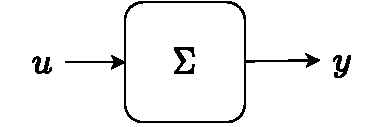
\includegraphics[width=0.35\textwidth]{figures/system}
    \end{figure}
    \begin{itemize}
      \item Linearity:
            \[
              \Sigma(\alpha u_1 + u_2)=\alpha\Sigma(u_1)+\Sigma(u_2),\quad\alpha \in \mathbb{R}
            \]
      \item Time-invariance:
            \[
              \Sigma\mathcal{S}_{\tau}(u) = \mathcal{S}_{\tau}\Sigma(u)
            \]
    \end{itemize}
    Dynamics of LTI systems are fully described by impulse response
    $h = \Sigma(\delta) \in \mathcal{L}_2(\mathbb{R})$:
    \begin{itemize}
      \item Convolution:
            \[
              \Sigma(u(t)) = (h \ast u)(t)
                           = \int_{-\infty}^\infty h(t - \tau)u(\tau)d\tau
                           = y(t)
            \]
    \end{itemize}
  }
  \only<2>
  {
    Let $u,y \in \blue{\ell_2(\mathbb{Z})}$, a system
    \(\Sigma:\blue{\ell_2(\mathbb{Z})} \rightarrow \blue{\ell_2(\mathbb{Z})}\)
    is a mapping $\Sigma(u) \mapsto y$
    \begin{figure}
      \centering 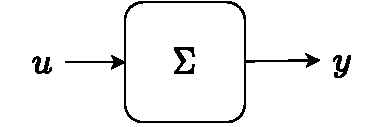
\includegraphics[width=0.35\textwidth]{figures/system}
    \end{figure}
    \begin{itemize}
      \item Linearity:
            \[
              \Sigma(\alpha u_1 + u_2)=\alpha\Sigma(u_1)+\Sigma(u_2),\quad\alpha \in \mathbb{R}
            \]
      \item Time-invariance:
            \[
              \Sigma\mathcal{S}_{\tau}(u) = \mathcal{S}_{\tau}\Sigma(u)
            \]
    \end{itemize}
    Dynamics of LTI systems are fully described by impulse response
    $h = \Sigma(\delta) \in \blue{\ell_2(\mathbb{Z})}$:
    \begin{itemize}
      \item Convolution:
            \[
              \Sigma(u(t)) = (h \ast u)(t) = \blue{\sum_{k\in\mathbb{Z}}h(t-k)u(k)} = y(t)
            \]
    \end{itemize}
  }
\end{frame}

\begin{frame}
  \frametitle{Frequency Domain Description} \(z\)-transform of impulse response:
  \[
    \mathcal{Z}\{h(t)\} = H(z) = \sum_{k \in \mathbb{Z}}h(k)z^{-k}
  \]
  Transmission is given by transfer function \(H(z)\):
  \[
    Y(z) = \mathcal{Z}\{y(t)\}
         = \mathcal{Z}\{h(t)\}
           \cdot \mathcal{Z}\{u(t)\}
         = H(z)
           \cdot U(z)
  \]
  Common representations:
  \begin{itemize}
    \item Rational:
          \[
            H(z) = \frac{\sum_{k=0}^{N}b_kz^{-k}}{1-\sum_{k=1}^{M}a_{k}z^{-k}}\onslide
                 < 2
                 > {\quad \rightarrow \quad\text{barycentric
          form}\footcite{trefethen2013}:~\frac{\sum_{k=0}^{K}\frac{\alpha_{k}}{z-t_k}}{\sum_{k=0}^K\frac{\beta_k}{z-t_k}}}
          \]
    \item Pole-residue:
          \[
            H(z) = \sum_{k = 1}^{K}\frac{c_kb_k}{z-\lambda_k}
          \]
  \end{itemize}
\end{frame}
%
\begin{frame}
  \frametitle{Hankel Singular Values}
  \vfill
  \centering
  \includegraphics{hsv-map.pdf}
  \includegraphics{hsv-colorbar.pdf}
  \vfill
\end{frame}
%
\begin{frame}
  \frametitle{Hankel Singular Values: ITD removed}
  \vfill
  \centering
  \includegraphics{hsv-map-itd-removed.pdf}
  \includegraphics{hsv-colorbar.pdf}
  \vfill
\end{frame}
%
\begin{frame}
  \frametitle{Relative Error}
  \vfill
  \centering
  \includegraphics[width=.6\textwidth]{bound-error.pdf}
  \includegraphics[width=.5\textwidth]{bound-error-legend.pdf}
  \vfill
\end{frame}
%
\begin{frame}[allowframebreaks]{References}
  \footnotesize \printbibliography
\end{frame}
%
\end{document}
